\documentclass[a4paper,11pt,exos]{nsi} % COMPILE WITH DRAFT


\pagestyle{empty}
\begin{document}

%Exercice 1E12


\subsection*{NOM, Prénom : \dotfill} 

\classe{\premiere spé}
\titre{Ceinture bleue 02 - Corrigé}
\maketitle

\begin{exercice}[ : Trouver l'équation d'une parabole]
    Quelle est l'expression de la fonction polynomiale $f$ du second degré qui s'annule en $x=-2$ et en $x=5$ et dont la parabole passe par le point de coordonnées $(0;20)$ ?\\
    Donner la forme développée de $f$.\\

    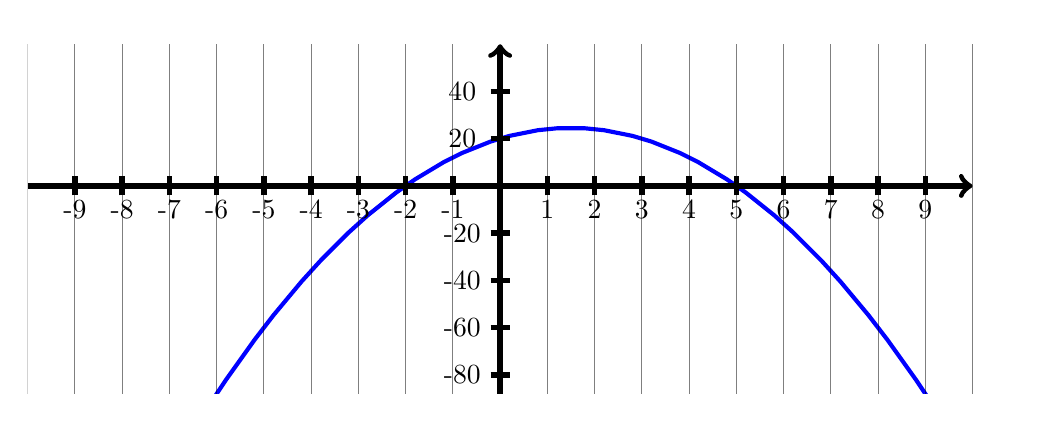
\begin{tikzpicture}[baseline,scale = 0.6]

        \tikzset{
          point/.style={
            thick,
            draw,
            cross out,
            inner sep=0pt,
            minimum width=5pt,
            minimum height=5pt,
          },
        }
        \clip (-10,-4.4) rectangle (11,3.35);
            
        \draw[color={blue},line width = 1.5] ;
        \draw[color={blue},line width = 1.5] ;
        \draw[color={blue},line width = 1.5] ;
        \draw[color={blue},line width = 1.5] ;
        \draw[color={blue},line width = 1.5] ;
        \draw[color={blue},line width = 1.5] ;
        \draw[color={blue},line width = 1.5] ;
        \draw[color={blue},line width = 1.5] ;
        \draw[color={blue},line width = 1.5] ;
        \draw[color={blue},line width = 1.5] ;
        \draw[color={blue},line width = 1.5] ;
        \draw[color={blue},line width = 1.5] ;
        \draw[color={blue},line width = 1.5] ;
        \draw[color={blue},line width = 1.5] ;
        \draw[color={blue},line width = 1.5] ;
        \draw[color={blue},line width = 1.5] (-7,-6)--(-6.8,-5.66)--(-6.6,-5.34)--(-6.4,-5.02)--(-6.2,-4.7)--(-6,-4.4)--(-5.8,-4.1)--(-5.6,-3.82)--(-5.4,-3.54)--(-5.2,-3.26)--(-5,-3)--(-4.8,-2.74)--(-4.6,-2.5)--(-4.4,-2.26)--(-4.2,-2.02)--(-4,-1.8)--(-3.8,-1.58)--(-3.6,-1.38)--(-3.4,-1.18)--(-3.2,-0.98)--(-3,-0.8)--(-2.8,-0.62)--(-2.6,-0.46)--(-2.4,-0.3)--(-2.2,-0.14)--(-2,0)--(-1.8,0.14)--(-1.6,0.26)--(-1.4,0.38)--(-1.2,0.5)--(-1,0.6)--(-0.8,0.7)--(-0.6,0.78)--(-0.4,0.86)--(-0.2,0.94)--(0,1)--(0.2,1.06)--(0.4,1.1)--(0.6,1.14)--(0.8,1.18)--(1,1.2)--(1.2,1.22)--(1.4,1.22)--(1.6,1.22)--(1.8,1.22)--(2,1.2)--(2.2,1.18)--(2.4,1.14)--(2.6,1.1)--(2.8,1.06)--(3,1)--(3.2,0.94)--(3.4,0.86)--(3.6,0.78)--(3.8,0.7)--(4,0.6)--(4.2,0.5)--(4.4,0.38)--(4.6,0.26)--(4.8,0.14)--(5,0)--(5.2,-0.14)--(5.4,-0.3)--(5.6,-0.46)--(5.8,-0.62)--(6,-0.8)--(6.2,-0.98)--(6.4,-1.18)--(6.6,-1.38)--(6.8,-1.58)--(7,-1.8)--(7.2,-2.02)--(7.4,-2.26)--(7.6,-2.5)--(7.8,-2.74)--(8,-3)--(8.2,-3.26)--(8.4,-3.54)--(8.6,-3.82)--(8.8,-4.1)--(9,-4.4)--(9.2,-4.7)--(9.4,-5.02)--(9.6,-5.34)--(9.8,-5.66)--(10,-6);
        
        \draw[color ={black},line width = 2,->] (-10,0)--(10,0);
        \draw[color ={black},line width = 2,->] (0,-6)--(0,3);
        \draw[color ={black},opacity = 0.5] (1,-6)--(1,3);
        \draw[color ={black},opacity = 0.5] (2,-6)--(2,3);
        \draw[color ={black},opacity = 0.5] (3,-6)--(3,3);
        \draw[color ={black},opacity = 0.5] (4,-6)--(4,3);
        \draw[color ={black},opacity = 0.5] (5,-6)--(5,3);
        \draw[color ={black},opacity = 0.5] (6,-6)--(6,3);
        \draw[color ={black},opacity = 0.5] (7,-6)--(7,3);
        \draw[color ={black},opacity = 0.5] (8,-6)--(8,3);
        \draw[color ={black},opacity = 0.5] (9,-6)--(9,3);
        \draw[color ={black},opacity = 0.5] (10,-6)--(10,3);
        \draw[color ={black},opacity = 0.5] (-1,-6)--(-1,3);
        \draw[color ={black},opacity = 0.5] (-2,-6)--(-2,3);
        \draw[color ={black},opacity = 0.5] (-3,-6)--(-3,3);
        \draw[color ={black},opacity = 0.5] (-4,-6)--(-4,3);
        \draw[color ={black},opacity = 0.5] (-5,-6)--(-5,3);
        \draw[color ={black},opacity = 0.5] (-6,-6)--(-6,3);
        \draw[color ={black},opacity = 0.5] (-7,-6)--(-7,3);
        \draw[color ={black},opacity = 0.5] (-8,-6)--(-8,3);
        \draw[color ={black},opacity = 0.5] (-9,-6)--(-9,3);
        \draw[color ={black},opacity = 0.5] (-10,-6)--(-10,3);
        \draw[color ={black},line width = 2] (1,-0.2)--(1,0.2);
        \draw[color ={black},line width = 2] (2,-0.2)--(2,0.2);
        \draw[color ={black},line width = 2] (3,-0.2)--(3,0.2);
        \draw[color ={black},line width = 2] (4,-0.2)--(4,0.2);
        \draw[color ={black},line width = 2] (5,-0.2)--(5,0.2);
        \draw[color ={black},line width = 2] (6,-0.2)--(6,0.2);
        \draw[color ={black},line width = 2] (7,-0.2)--(7,0.2);
        \draw[color ={black},line width = 2] (8,-0.2)--(8,0.2);
        \draw[color ={black},line width = 2] (9,-0.2)--(9,0.2);
        \draw[color ={black},line width = 2] (-1,-0.2)--(-1,0.2);
        \draw[color ={black},line width = 2] (-2,-0.2)--(-2,0.2);
        \draw[color ={black},line width = 2] (-3,-0.2)--(-3,0.2);
        \draw[color ={black},line width = 2] (-4,-0.2)--(-4,0.2);
        \draw[color ={black},line width = 2] (-5,-0.2)--(-5,0.2);
        \draw[color ={black},line width = 2] (-6,-0.2)--(-6,0.2);
        \draw[color ={black},line width = 2] (-7,-0.2)--(-7,0.2);
        \draw[color ={black},line width = 2] (-8,-0.2)--(-8,0.2);
        \draw[color ={black},line width = 2] (-9,-0.2)--(-9,0.2);
        \draw[color ={black},line width = 2] (-0.2,1)--(0.2,1);
        \draw[color ={black},line width = 2] (-0.2,2)--(0.2,2);
        \draw[color ={black},line width = 2] (-0.2,-1)--(0.2,-1);
        \draw[color ={black},line width = 2] (-0.2,-2)--(0.2,-2);
        \draw[color ={black},line width = 2] (-0.2,-3)--(0.2,-3);
        \draw[color ={black},line width = 2] (-0.2,-4)--(0.2,-4);
        \draw[color ={black},line width = 2] (-0.2,-5)--(0.2,-5);
        \draw [color={black},fill opacity = 1] (1,-0.5) node[anchor = center,scale=1] {1};
        \draw [color={black},fill opacity = 1] (2,-0.5) node[anchor = center,scale=1] {2};
        \draw [color={black},fill opacity = 1] (3,-0.5) node[anchor = center,scale=1] {3};
        \draw [color={black},fill opacity = 1] (4,-0.5) node[anchor = center,scale=1] {4};
        \draw [color={black},fill opacity = 1] (5,-0.5) node[anchor = center,scale=1] {5};
        \draw [color={black},fill opacity = 1] (6,-0.5) node[anchor = center,scale=1] {6};
        \draw [color={black},fill opacity = 1] (7,-0.5) node[anchor = center,scale=1] {7};
        \draw [color={black},fill opacity = 1] (8,-0.5) node[anchor = center,scale=1] {8};
        \draw [color={black},fill opacity = 1] (9,-0.5) node[anchor = center,scale=1] {9};
        \draw [color={black},fill opacity = 1] (-1,-0.5) node[anchor = center,scale=1] {-1};
        \draw [color={black},fill opacity = 1] (-2,-0.5) node[anchor = center,scale=1] {-2};
        \draw [color={black},fill opacity = 1] (-3,-0.5) node[anchor = center,scale=1] {-3};
        \draw [color={black},fill opacity = 1] (-4,-0.5) node[anchor = center,scale=1] {-4};
        \draw [color={black},fill opacity = 1] (-5,-0.5) node[anchor = center,scale=1] {-5};
        \draw [color={black},fill opacity = 1] (-6,-0.5) node[anchor = center,scale=1] {-6};
        \draw [color={black},fill opacity = 1] (-7,-0.5) node[anchor = center,scale=1] {-7};
        \draw [color={black},fill opacity = 1] (-8,-0.5) node[anchor = center,scale=1] {-8};
        \draw [color={black},fill opacity = 1] (-9,-0.5) node[anchor = center,scale=1] {-9};
        \draw [color={black},fill opacity = 1] (-0.8,1) node[anchor = center,scale=1] {20};
        \draw [color={black},fill opacity = 1] (-0.8,2) node[anchor = center,scale=1] {40};
        \draw [color={black},fill opacity = 1] (-0.8,-1) node[anchor = center,scale=1] {-20};
        \draw [color={black},fill opacity = 1] (-0.8,-2) node[anchor = center,scale=1] {-40};
        \draw [color={black},fill opacity = 1] (-0.8,-3) node[anchor = center,scale=1] {-60};
        \draw [color={black},fill opacity = 1] (-0.8,-4) node[anchor = center,scale=1] {-80};
        \draw [color={black},fill opacity = 1] (-0.8,-5) node[anchor = center,scale=1] {-100};
    
    \end{tikzpicture}\\
\end{exercice}


Comme $-2$ et $5$ sont les deux solutions de l'équation $f(x)=0$, on peut factoriser $f(x)$ :\\$f(x)=a(x+2)(x-5)$.\\[.5em]
Comme $f(0)=20$, on en déduit que $20=a(0+2)(0-5)$ d'où $a=20\div (-10)=-2$.\\[.5em]
On obtient ainsi $f(x)=-2(x+2)(x-5)$ ou en développant $f(x)=-2x^2 +6x  +20$

\end{document}